% =====================================================================
%  body.tex  —  Fine-Grained Computation Offload for Event-Driven Applications
% =====================================================================

\section{Introduction}
\label{sec:intro}

Hardware accelerators are now a standard part of online serving. GPUs, TPUs, and FPGAs accelerate
machine-learning inference, image processing, encryption, and compression, and an increasing share
of ``acceleration'' is in fact a \emph{remote} call: to a hardware security module that signs a
token, to a post-quantum key-encapsulation service~\cite{mlkem}, or to a co-located inference
server~\cite{clipper}. The shape of
the application is remarkably uniform across these cases. A server receives a request from the
network, does some pre-processing, invokes a computationally intensive routine, does some
post-processing, and sends a response. When the intensive routine runs on an accelerator, it is
replaced by an \emph{offload}: a submission to the device and a wait for its completion. This raises
a deceptively simple question that this paper is about: \emph{what should the CPU do while it waits
for the accelerator?}

\begin{figure}[t]
  \centering
  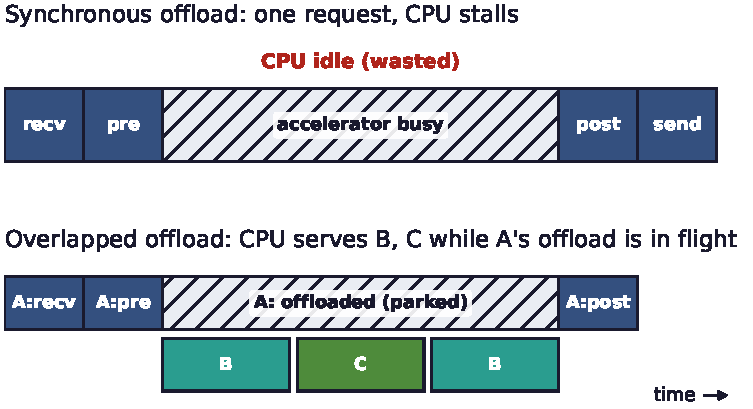
\includegraphics[width=\linewidth]{figs/fig_pipeline.pdf}
  \caption{The problem. A serving request is \emph{receive $\to$ pre-process $\to$ offload $\to$
    post-process $\to$ send}. Top: with a synchronous offload, the CPU stalls while the accelerator
    works. For fine-grained offloads (microseconds to a few milliseconds), a context switch to fill
    the gap costs as much as the gap itself, and busy-waiting wastes the core. Bottom: \emph{overlap}
    fills the gap with other requests' processing. The question of this paper is how much an existing
    server must change to do this.}
  \label{fig:pipeline}
\end{figure}

The textbook answers are unsatisfying precisely in the regime that matters
(Figure~\ref{fig:pipeline}). The first is to \emph{relinquish the CPU}: after submitting the
offload, block, and let the operating system run another thread. But a context switch on Linux costs
several microseconds, and a fine-grained offload, whether AES on a few kilobytes, a small inference,
or an HSM round-trip, also takes from a few to tens of microseconds. This is the
``killer microsecond'' regime~\cite{microsecond}: too long to spin away, too short for the operating
system to schedule around profitably. The switch overhead is then comparable
to the work it overlaps. It wastes CPU and \emph{adds} a thread-wakeup delay to the request's tail
latency. The second answer is to \emph{busy-wait} on the completion flag, which hides the wakeup
delay but burns a core doing nothing. The third, and the only principled one, is to \emph{do other
useful work} on the same CPU while the offload is in flight. This means \emph{overlapping} the offload
with the processing of other requests. It is what high-performance systems already do by hand. The
difficulty is that overlapping requires \emph{concurrency} inside the application at the offload
point, and existing servers express concurrency in many different ways. The central question of this
paper is therefore not \emph{whether} to overlap, but \emph{how much an off-the-shelf server must be
changed to do so}.

We answer this empirically, across the landscape of real servers, and the answer is a
\textbf{spectrum} bounded by two extremes (Figure~\ref{fig:spectrum}). At one extreme, overlap can be
injected with \emph{no source modification at all}. We build a user-space M:N fiber runtime, loaded
by \texttt{LD\_PRELOAD}, that interposes the standard threading and I/O symbols: it turns each
connection-handling thread into a lightweight fiber, yields the fiber at every blocking point, and
runs other fibers on the same core in the meantime. On a synchronous thread-per-connection handler
it delivers large speedups, $17.3\times$ over a synchronous baseline for GPU AES, with the
application binary unchanged. But transparency reaches only so far, and mapping exactly how far is
itself a contribution. Running the runtime under stock binaries surfaces a sequence of obstacles that
any threading-interposing tool must solve (most notably a glibc condition-variable symbol-versioning
hazard that silently corrupts some binaries). Beyond those lie \emph{three architectural walls}
that no engineering removes: storage engines that synchronize with raw \texttt{futex} system calls
\emph{below} the libc interface, managed runtimes that store thread identity in a native
thread-local slot the loader cannot virtualize, and workloads whose per-request CPU already exceeds
the offload so that there is no idle time to reclaim. Crucially, the runtime engages only on
\emph{thread-per-connection} servers. An event-driven server has a single event loop and no
per-connection thread to fiberize. So the very class of applications with the \emph{most} to gain
from overlap, where one synchronous offload stalls the \emph{entire} server, is the class transparency
cannot help.

At the other extreme, overlap can be injected with \emph{a few lines}. The recipe is uniform:
replace the synchronous offload at its call site with an asynchronous one that hands the work to the
application's \emph{own} concurrency mechanism, such as a module's background thread pool, an event
loop's deferred-response primitive, or a language runtime's tasks. The request is then answered on
completion. The edit is small because every modern server already contains machinery to suspend and
resume work. One only has to route the offload through it. We instantiate this recipe on \textbf{ten}
off-the-shelf servers spanning every concurrency model: Redis, nginx, memcached, Node.js,
Python/asyncio, Apache, Go, PostgreSQL, MariaDB, and HAProxy. In each case the change is \textbf{18 to
112 lines added, and zero or one existing line modified}. Measured on real hardware throughout, with
no emulated latencies, the edit recovers $1.2$--$5\times$ with no failed requests
(Figure~\ref{fig:headline}). It is bounded at
both ends, by the accelerator's throughput and by how much concurrency the server can itself express
(\S\ref{sec:eval}).

Behind these numbers is a simple predictive model, the paper's main intellectual contribution. Two
properties of a server fix both the speedup \emph{and} the code cost of overlapping an offload: its
\emph{concurrency model}, which places it in a regime that predicts how much a minimal edit buys and
how many lines it takes (dominated by whether the server already exposes a deferred-response
primitive), and the offload's \emph{weight relative to per-request CPU}, which predicts whether overlap
helps at all. The model explains the full range of our measurements, including where overlap does
\emph{not} help, and tells an operator in advance which servers to touch and what to expect.

Overlap also introduces one correctness hazard. When the post-processing after an offload mutates
shared state, overlapping two requests can reorder their read-modify-write sequences and corrupt it. We
provide a transparent conflict detector, based on page protection and version snapshots, that flags
exactly these conflicts and serializes only the conflicting work, at both ends of the spectrum and with
no application annotation.

In summary, this paper makes the following contributions:
\begin{itemize}[leftmargin=1.4em,itemsep=2pt,topsep=2pt]
  \item \textbf{A predictive model} of fine-grained offload overlap in existing servers: speedup and
    code cost as a function of the server's concurrency model and the offload's weight relative to
    per-request work, validated across ten real servers (\S\ref{sec:taxonomy}).
  \item \textbf{The transparent boundary, characterized}: a zero-modification M:N fiber runtime, the
    obstacle taxonomy it must overcome (including a reusable glibc condition-variable versioning
    bug), three architectural walls where transparency provably stops, and a classifier that predicts
    whether a binary is fiberizable (\S\ref{sec:transparent}).
  \item \textbf{A minimal-edit recipe and a cross-landscape study}: one offload-overlap pattern on
    ten off-the-shelf servers with 18--112 lines added and 0--1 lines modified, evaluated on real
    hardware ($1.2$--$5\times$). We also find that the win is bounded at both ends: by the
    accelerator's throughput (a large GPU offload saturates the device's bandwidth) and by the
    server's own overlap capacity (a real latency-bound remote signer tops out at $3.5\times$ behind a
    GIL-bound executor)
    (\S\ref{sec:minimal}, \S\ref{sec:eval}).
  \item \textbf{A transparent conflict detector} that keeps overlapped offload correct when it
    mutates shared state, with no application changes (\S\ref{sec:correctness}).
\end{itemize}


% =====================================================================
\section{Background and Motivation}
\label{sec:background}

\paragraph{Accelerators and the fine-grained regime.}
An accelerator turns a CPU-bound routine into a device operation: the CPU prepares an input buffer,
submits it (a kernel launch, a DMA, or a network send), and later collects the result. These
round-trips span microseconds to milliseconds (Figure~\ref{fig:landscape}), but what unites them is
that they are \emph{fine-grained} relative to operating-system scheduling: the offload finishes on a
timescale comparable to a context switch. There the classic ways of waiting are wasteful
(Figure~\ref{fig:pipeline})---blocking pays a switch and a wakeup that rival the offload, busy-waiting
burns a core---so overlapping the offload with other work is the only approach that neither wastes the
CPU nor inflates latency.

\begin{figure}[t]
  \centering
  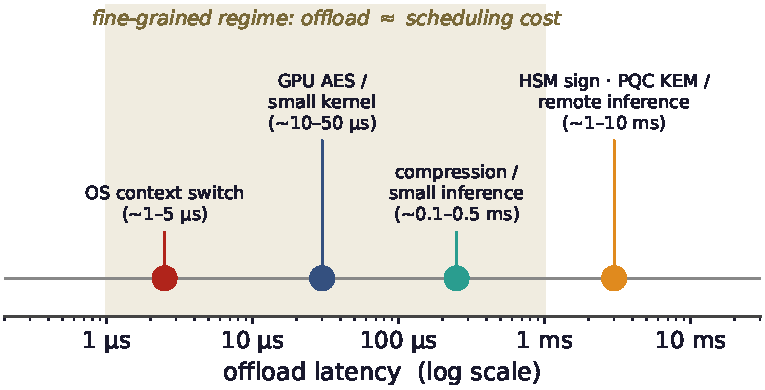
\includegraphics[width=\linewidth]{figs/fig_landscape.pdf}
  \caption{The fine-grained regime. Accelerator offloads span microseconds to milliseconds. In the
    shaded band, the offload latency is comparable to an OS context switch, so blocking pays a switch
    and a wakeup that rival the work itself, and busy-waiting wastes a core. This is exactly where
    overlapping the offload with other requests is the right answer.}
  \label{fig:landscape}
\end{figure}

\paragraph{How servers express concurrency.}
``Other work to overlap with'' means \emph{concurrent requests}, and a server's ability to overlap an
offload is determined by how it runs concurrent requests in the first place. We find it useful to
group servers into a few models, which recur throughout the paper. A \emph{single-event-loop} server
(e.g., Redis, Node.js, a Python \texttt{asyncio} service) multiplexes all connections on one thread
that loops over ready events. An \emph{event-loop-with-pool} server (nginx, memcached) runs a few
such loops plus a worker pool for blocking work. A \emph{thread- or goroutine-pool} server (Apache,
Go) dispatches each request to a pooled worker or a runtime-scheduled task. A \emph{proxy} (HAProxy)
forwards each request through a native offload engine rather than running application logic itself.
A \emph{process- or thread-per-connection} server (PostgreSQL, MariaDB) gives each connection its
own backend. These models differ sharply in what a synchronous offload \emph{costs} and in how overlap
must be injected, differences this paper turns into a predictive model (\S\ref{sec:taxonomy}).

\paragraph{The motivating catastrophe.}
The starkest case is a single event loop: because one thread handles every connection, a synchronous
offload blocks \emph{all} connections for its full duration, and throughput collapses to one request
per offload latency while the hardware sits idle---a pathology of \emph{structure}, not capacity. A
few lines that move the offload off the loop recover more than an order of magnitude (\S\ref{sec:eval}).
The event-driven servers that dominate modern serving thus have the most to gain from overlap and, as
we show next, are also the ones a transparent runtime cannot help.


% =====================================================================
\section{Transparent Overlap: The Zero-Edit Extreme}
\label{sec:transparent}

We begin at the zero-modification end of the spectrum. The goal is the most convenient form of
overlap imaginable: take an \emph{unmodified} server binary and make it overlap its offloads, with no
recompilation and no source access. The result is an existence proof that the mechanism works. More
importantly for the rest of the paper, it is a precise map of how far transparency can reach.

\subsection{An \texttt{LD\_PRELOAD} M:N fiber runtime}

Our runtime (Figure~\ref{fig:runtime}) is a shared library loaded ahead of the application by
\texttt{LD\_PRELOAD}. It interposes the standard threading and I/O symbols. When the application
creates a connection-handling thread, the runtime instead spawns a \emph{fiber}: a user-level thread
with its own small stack and a hand-written, register-only context switch of tens of nanoseconds,
some twenty times cheaper than a kernel switch~\cite{fastwake}. All fibers run on a single
\emph{carrier} OS thread.
When a fiber would block, whether on a socket read or write or on the offload, the runtime saves its
context and switches to another runnable fiber. A scheduler on the carrier waits for I/O readiness
and offload completions and resumes the corresponding fiber. The application's handler keeps its
plain, synchronous shape: read a request, call the offload, write a reply. It never learns that its
``thread'' is a fiber or that its offload was overlapped with its neighbors'. Per-fiber state that
the C library treats as thread-local, such as \texttt{errno} and the OpenSSL error queue, is saved
and restored at every switch so that fibers do not see each other's transient state.

\begin{figure}[t]
  \centering
  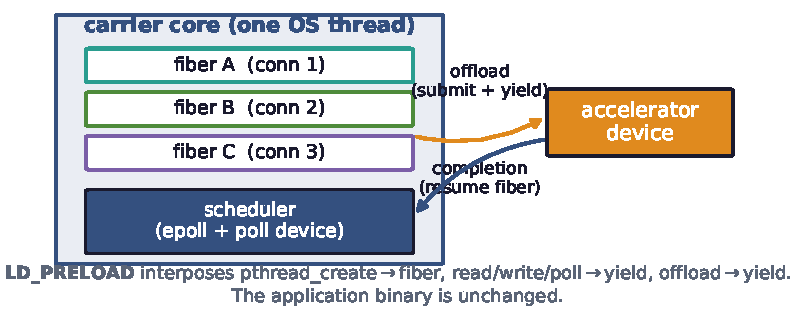
\includegraphics[width=0.92\linewidth]{figs/fig_runtime.pdf}
  \caption{The transparent runtime. An \texttt{LD\_PRELOAD} library turns each connection thread into
    a fiber on one carrier core. A fiber yields at its offload (and at socket I/O), and the scheduler
    runs another fiber until the device completes. The application binary is unchanged. On a
    synchronous thread-per-connection handler with a real GPU this overlaps 64 connections' offloads
    and delivers $17.3\times$ over a blocking baseline.}
  \label{fig:runtime}
\end{figure}

On a synchronous thread-per-connection handler this works well. With a real GPU performing AES, the
runtime overlaps 64 connections' offloads on one carrier core and reaches $17.3\times$ the throughput
of the same binary blocking on each offload, with results verified bit-for-bit. A DNN-inference
server shows $11.8\times$. These results confirm the mechanism. The rest of this section is about its limits,
which turn out to be the more useful contribution.

\subsection{What it takes to run real binaries}

Interposing the threading layer of a stock binary is harder than it sounds. The sharpest obstacle is a
\emph{symbol-versioning} hazard~\cite{drepper}: the glibc condition-variable functions carry two
incompatible ABIs under one name, so a naive interposer that defines an \emph{unversioned}
\texttt{pthread\_cond\_signal} breaks the linker's version-matched relocation and silently corrupts
some binaries (MariaDB crashes at startup with a wild pointer) while sparing others
(Figure~\ref{fig:condsweep}). The fix is to export the interposed symbols at their exact version and
resolve the real ones with \texttt{dlvsym}. The defect is latent in any threading-interposing tool, a
reusable practitioner lesson. Several lesser obstacles---alternate I/O entry points, real-thread
identity for libc's stack-bounds logic, carrier re-establishment after a daemon's \texttt{fork}, and
priority inversion under real-time pinning---we resolved once each; Appendix~\ref{app:obstacles}
records them.

\begin{figure}[t]
  \centering
  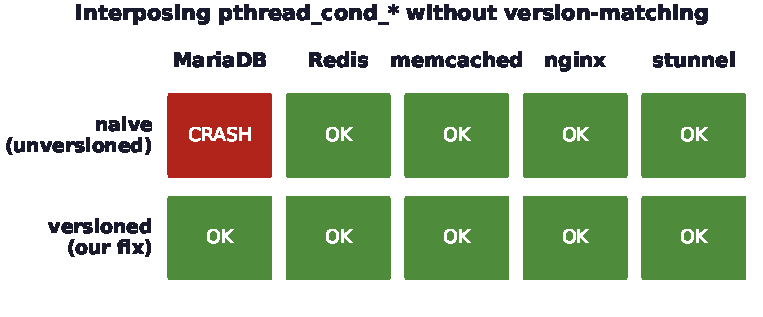
\includegraphics[width=0.9\linewidth]{figs/fig_condsweep.pdf}
  \caption{A reusable interposition hazard. The glibc condition-variable functions carry two
    incompatible ABIs under one name. A naive unversioned interposer breaks the version-matched
    relocation and corrupts \emph{some} binaries (MariaDB crashes at startup) while silently sparing
    others. Version-matching the interposed symbols fixes all of them. Any threading-interposing tool
    must do this.}
  \label{fig:condsweep}
\end{figure}

\subsection{Three walls where transparency stops}

Beyond engineering obstacles lie three \emph{walls} that no amount of interposition removes
(Figure~\ref{fig:walls}). Each is a place where the application's behavior escapes the layer a
preloaded library can intercept.

\emph{Wall 1: synchronization below libc.} A storage engine such as InnoDB does its internal
locking with the \texttt{futex} system call~\cite{futexes} issued \emph{directly}, bypassing the
\texttt{pthread} layer entirely. A userspace runtime interposes library \emph{symbols}, not system
calls. A fiber that blocks in a raw \texttt{futex} therefore stalls the entire carrier, and under
contention the whole server deadlocks. We confirmed this with a live backtrace of the frozen carrier inside InnoDB's
synchronization code.

\emph{Wall 2: thread identity in native TLS.} A managed runtime such as the JVM stores ``the current
thread'' in a native thread-local slot read directly from a CPU register, not through any library
call. Fibers that share one carrier OS thread cannot be given distinct values of that slot by symbol
interposition, so after a fiber switch the runtime reads the \emph{wrong} thread object and
segfaults. We observe exactly this: a crash dereferencing a stale \texttt{Thread*} the moment two
fiberized JVM requests interleave. The same mechanism applies to Go and .NET.

\emph{Wall 3: no idle CPU to reclaim.} Overlap only helps if the CPU is idle during the offload. A
TLS terminator that is already thread-per-connection and spends real CPU on per-request crypto has no
such idle time: the OS already overlaps its offloads across threads, while the single carrier
serializes the real crypto and pays an interposition tax on every yield. The result is $2$--$3\times$
\emph{slower} than native on the same core.

\begin{figure}[t]
  \centering
  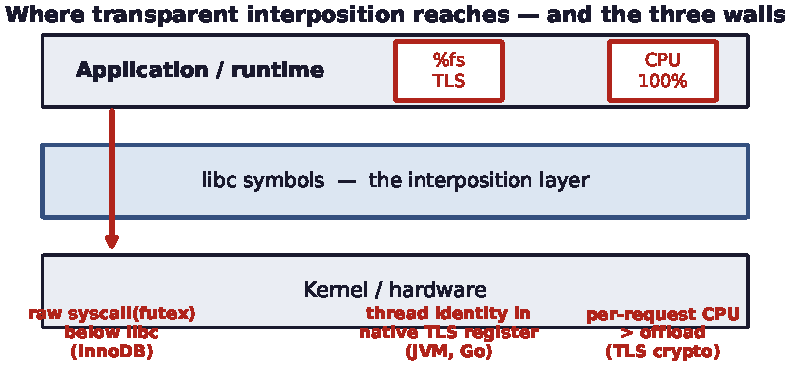
\includegraphics[width=\linewidth]{figs/fig_walls.pdf}
  \caption{The three walls. Transparent interposition virtualizes the libc symbol layer
    (read/write, the \texttt{pthread} primitives, \texttt{errno}). It cannot reach three things. The
    first is synchronization issued as a \emph{raw} system call below libc (InnoDB's \texttt{futex}).
    The second is thread identity held in a native TLS register (the JVM, Go). The third is a workload
    where per-request CPU already exceeds the offload, leaving no idle time. These bound where
    zero-edit overlap is possible.}
  \label{fig:walls}
\end{figure}

\subsection{A classifier for fiberizability}

The walls are not arbitrary. They are predictable from a binary's behavior. We profile the
\emph{per-request blocking syscalls} a server makes under load. Event-driven servers do their I/O
with \texttt{epoll} and \texttt{read} and have no per-connection thread to fiberize: the runtime
loads safely but never engages. Thread-per-connection servers whose blocking is all at the libc layer
have \emph{near-zero} per-request \texttt{futex} traffic and are fiberizable. Engines that
synchronize below libc have \texttt{futex} traffic that dominates their profile and use kernel-bypass
I/O such as \texttt{io\_uring}~\cite{iouring}. This is the wall. Figure~\ref{fig:classifier} makes it
concrete: InnoDB's per-request \texttt{futex} density is roughly two orders of magnitude above a
fiberizable server's, a cheap static-plus-dynamic check that tells an operator in advance whether a
binary can be fiberized.

\begin{figure}[t]
  \centering
  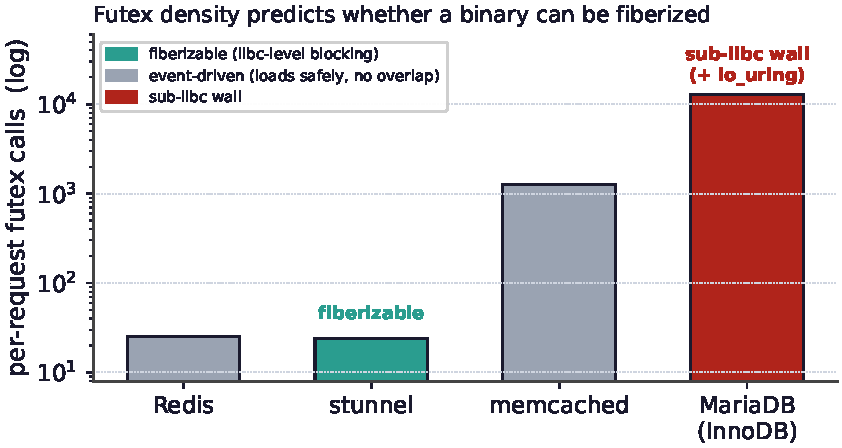
\includegraphics[width=0.86\linewidth]{figs/fig_classifier.pdf}
  \caption{Predicting fiberizability. Per-request \texttt{futex} calls separate the near-zero
    libc-level servers (whose blocking the runtime can interpose) from engines that synchronize below
    libc (InnoDB, $\sim$$13{,}000$, plus \texttt{io\_uring}), the wall of Figure~\ref{fig:walls}. The
    same profile flags event-driven servers as ``loads safely, no overlap.''}
  \label{fig:classifier}
\end{figure}

The verdict frames the rest of the paper. Transparency serves a narrow niche: thread-per-connection
servers with light per-request CPU and a libc-level offload. By construction, it cannot help
the event-driven servers that have the most to gain. For everyone else, a few lines suffice.


% =====================================================================
\section{Minimal-Edit Overlap}
\label{sec:minimal}

If a server cannot be fiberized from the outside, it can almost always be overlapped from a small
edit inside. The reason is that every modern server already contains the machinery to \emph{suspend}
a request and \emph{resume} it later. That machinery is what lets it serve many connections at
once. To overlap an offload, one only has to route it through that machinery instead of blocking on
it. The recipe is uniform across servers:

\begin{enumerate}[leftmargin=1.5em,itemsep=1pt,topsep=2pt]
  \item at the offload call site, \emph{submit} the work to a background executor instead of waiting.
  \item \emph{suspend} the current request using the server's own deferred-response primitive.
  \item \emph{resume} it and send the reply when the offload completes.
\end{enumerate}

\begin{figure}[t]
  \centering
  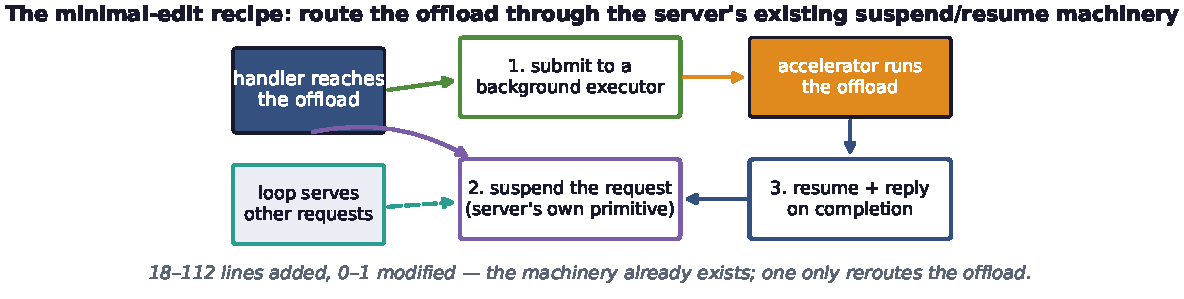
\includegraphics[width=\linewidth]{figs/fig_recipe.pdf}
  \caption{The minimal-edit recipe. At the offload call site, submit the work to a background
    executor, suspend the request with the server's own deferred-response primitive, and resume it
    to reply on completion. Meanwhile the server's loop serves other requests. The edit is small
    because the suspend/resume machinery already exists. One only reroutes the offload through it.}
  \label{fig:recipe}
\end{figure}

We distinguish two quantities: \emph{lines added} (the new integration code) and \emph{existing lines
modified} (edits to code already in the server). The second is the invasive, maintenance-costly part.
Zero is ideal and is achievable wherever the server exposes a plugin or extension interface. We
instantiate the recipe on ten servers spanning every concurrency model, and in every case the change is
\textbf{18--112 lines added and 0--1 lines modified} (Figure~\ref{fig:spectrum}).

\begin{figure}[t]
  \centering
  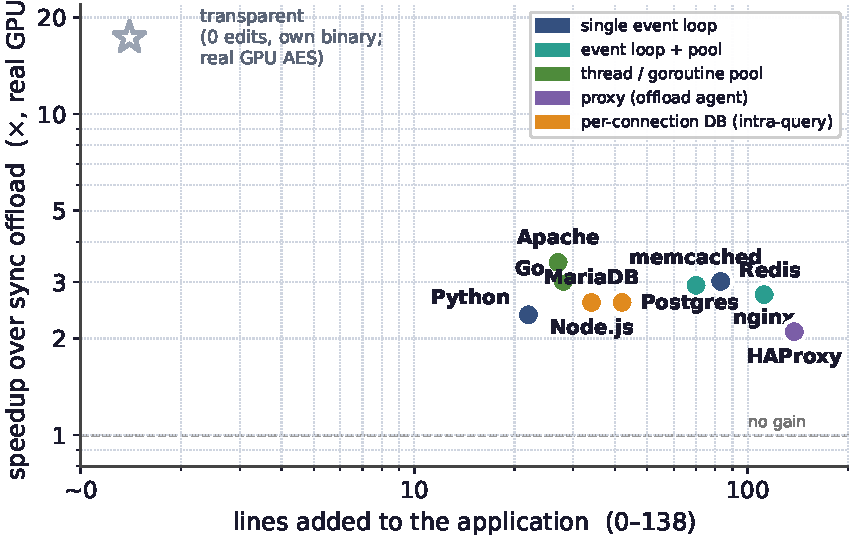
\includegraphics[width=\linewidth]{figs/fig_spectrum.pdf}
  \caption{The spectrum (the paper in one plot), all on a \emph{real GPU} with a $1$\,MiB AES offload,
    measured on an idle GPU. Each point is an off-the-shelf server. The $x$-axis is the lines of
    integration code, the $y$-axis the real-GPU speedup from overlapping the offload. The few-line
    edit clusters at $2$--$3.5\times$. A real bandwidth-bound GPU offload lets overlap fill the
    device but not exceed its throughput. The databases sit lower (intra-query pipelining only, as
    their backends already overlap across connections). HAProxy's proxy reaches $2.1\times$ with a
    C offload agent (a GIL-bound Python agent gets only $0.9\times$). The zero-line transparent
    runtime reaches $17.3\times$ in its niche on a small launch-bound offload (walls on third-party
    binaries). Color encodes the concurrency model (\S\ref{sec:taxonomy}).}
  \label{fig:spectrum}
\end{figure}

The integration point follows the concurrency model. Servers with a \emph{plugin or extension API}
take the recipe with zero core edits: a Redis~\cite{redis} module, an nginx~\cite{nginx} thread-pool
add-on, an Apache~\cite{apache} content handler, PostgreSQL~\cite{postgresql} and MariaDB~\cite{mariadb}
user-defined functions, a Node.js~\cite{nodejs} N-API addon over libuv~\cite{libuv}, and a
HAProxy~\cite{haproxy} deployment that streams each request to an external offload \emph{agent} over
its native SPOE engine~\cite{spoe}. Servers backed by a \emph{language runtime} need \emph{no
asynchronous code at all}: a Go~\cite{golang} handler's plain blocking \texttt{cgo} offload is
overlapped by the goroutine scheduler, and a Python \texttt{asyncio}~\cite{cpython} service offloads
through \texttt{run\_in\_executor} in one line. The lone case touching existing code is
memcached~\cite{memcached}, which has no asynchronous-command interface, so we add the park/resume
transition to its state machine (70 lines, one modified). memcached is the exception that proves the
rule: the line count is dominated by whether the server already exposes a deferred-response primitive,
which we formalize next.


% =====================================================================
\section{A Predictive Model of Offload Overlap}
\label{sec:taxonomy}

The measurements above are not a list of unrelated wins. They follow a pattern. Two properties of a
server predict both \emph{how much} overlap helps and \emph{how many lines} it takes: the server's
\emph{concurrency model} and the offload's \emph{weight relative to per-request CPU work}.

\paragraph{Concurrency model predicts the regime.}
Figure~\ref{fig:regimes} lays out the regimes, from \emph{dramatic} to \emph{none}. A \emph{single
event loop} is the extreme case---a synchronous offload stalls the whole server, so the few-line fix
restores full concurrency and the win grows with offload weight up to the throughput ceiling---while an
\emph{event loop with a worker pool} stalls only one loop of several. A \emph{thread or goroutine pool}
overlaps offloads \emph{automatically} with zero asynchronous code, and a \emph{proxy} with a native
offload engine makes async offload configuration-only. A \emph{process- or thread-per-connection}
server already overlaps \emph{across} connections for free (the OS runs the backends concurrently), so
its only edit-addressable win is \emph{within} a single query that pipelines a serial loop of offloads.

\begin{figure}[t]
  \centering
  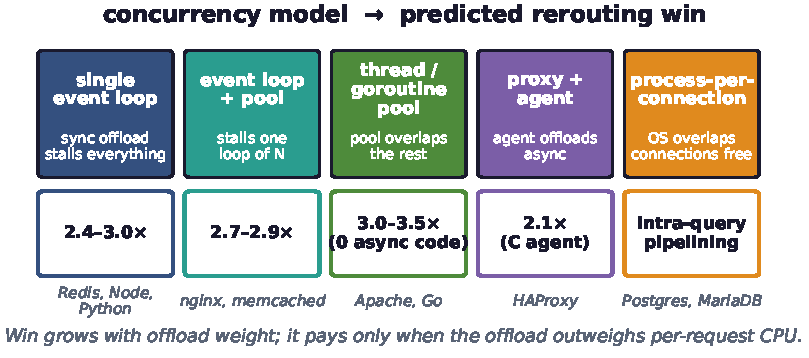
\includegraphics[width=\linewidth]{figs/fig_regimes.pdf}
  \caption{The predictive model, part one: the concurrency model determines what a synchronous
    offload costs and therefore how much a minimal edit recovers. The win ranges from
    \emph{dramatic} (a blocked single loop) to \emph{automatic} (a pool that overlaps for free) to
    \emph{intra-query} (databases that already overlap across connections). Example servers are shown
    under each regime.}
  \label{fig:regimes}
\end{figure}

\paragraph{Code cost follows the same axis.}
The number of lines is governed by whether the server exposes an asynchronous, deferred-response
primitive. Plugin and extension interfaces (Redis, nginx, Apache, the databases) and language
runtimes (Go, Python) provide one, so the integration is purely additive. No existing lines
change. A server without such a primitive forces the developer to add the suspend/resume transition
to its request state machine by hand. memcached is our only such case, and it is the only one that
modifies an existing line.

\paragraph{Offload weight predicts whether overlap helps at all.}
The second axis is independent of the server (Figure~\ref{fig:weight}). Overlap reclaims the wait for
the offload, so if per-request CPU work is already comparable to the offload there is little to
reclaim. A block-size sweep of a real GPU AES offload on a single event loop bears this out: a light
block yields essentially no speedup and the win grows monotonically with weight toward the GPU's
bandwidth (Figure~\ref{fig:weight}). The rule is simple and bounds applicability: overlap pays exactly
when the offload outweighs the per-request CPU work \emph{and} the accelerator is not already
saturated---the same condition as Wall~3 of \S\ref{sec:transparent}, seen from the transparent side.

\begin{figure}[t]
  \centering
  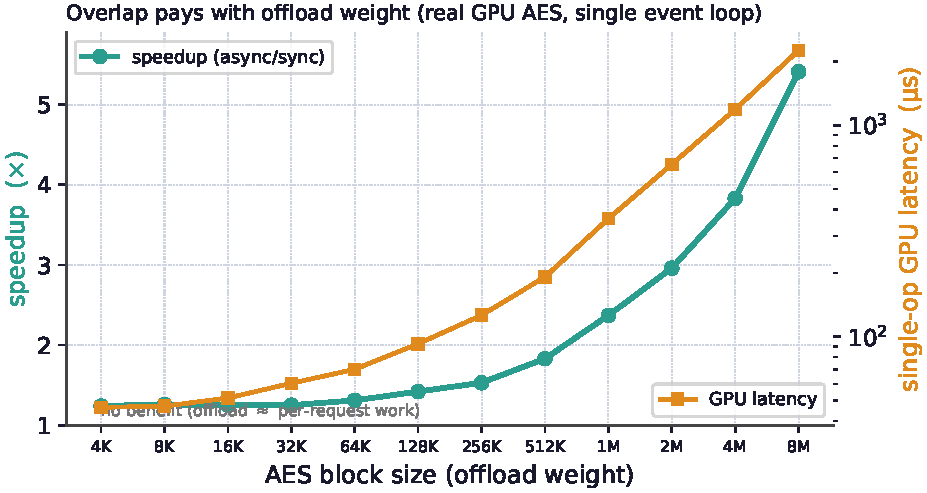
\includegraphics[width=0.86\linewidth]{figs/fig_weight.pdf}
  \caption{The predictive model, part two (measured, real GPU, idle): overlap pays only when the
    offload outweighs per-request CPU work. Sweeping a real GPU AES offload by block size
    (consecutive powers of two, $4$\,KiB--$8$\,MiB) on a single-event-loop server, the same edit gives
    no benefit for a light block ($1.24\times$ at $4$\,KiB, $46$\,\textmu s) and rises to $5.41\times$
    at $8$\,MiB ($2.3$\,ms), approaching the GPU's bandwidth. Right axis: measured single-op GPU
    latency. This condition also explains the transparent runtime's third wall.}
  \label{fig:weight}
\end{figure}

Together the two axes form a map: given a server's concurrency model and an offload's latency, one
can predict before writing any code whether to bother, how large the win will be, and roughly how
many lines it will take.


% =====================================================================
\section{Correctness: Overlapping Stateful Offloads}
\label{sec:correctness}

Overlap reorders work, and reordering is dangerous when the work touches shared state. If the
post-processing after an offload does a read-modify-write on a global---a counter, a cache entry, a key
in a store---overlapping two requests can interleave their sequences and lose updates. On a \emph{stock
Redis server} whose module command reads a key, runs a real GPU offload, and writes the incremented
value back, unprotected overlap silently loses tens of thousands of updates
(Figure~\ref{fig:correctness}, left). The hazard is subtle precisely because the offload widens the
read-modify-write window: the more latency overlap hides, the wider the race it opens.

Two mechanisms restore correctness with no application change. \emph{Per-connection ordering} is free:
one fiber per connection serializes a connection's dependent requests automatically. For state shared
\emph{across} connections we add a transparent \emph{conflict detector} that write-protects the
shared-state pages, snapshots a version clock when a handler parks at its offload, and treats a write
fault on a page modified during the park as a conflict; under enforcement it serializes only the
conflicting handlers while everyone else stays overlapped. On the stock-Redis workload it flags
essentially every conflict and drives lost updates to \emph{zero}, and it keeps overlap where a lock
would destroy it---running $1.8\times$ faster than a coarse lock that serializes the very offloads it
protects (Figure~\ref{fig:correctness}, right). The detector is a property of the overlap mechanism,
not of any one integration, so it applies to both ends of the spectrum.

\begin{figure}[t]
  \centering
  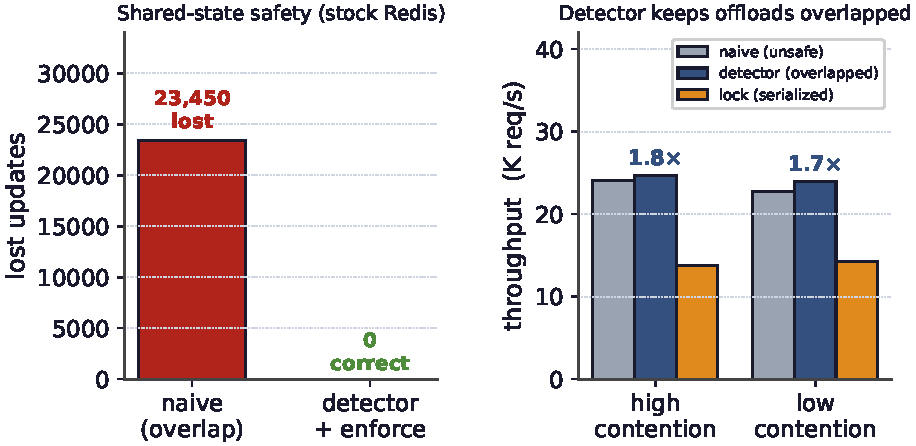
\includegraphics[width=\linewidth]{figs/fig_correctness.pdf}
  \caption{Keeping overlapped stateful offloads correct, measured on a stock Redis server with a real
    GPU offload. Left: unprotected overlap of a shared read-modify-write loses $23{,}450$ updates. The
    page-protection detector flags $26{,}185$ conflicts and, under enforcement, reduces lost updates
    to zero. Right: a coarse lock serializes the very offloads it protects ($13.8$K\,req/s), while the
    detector keeps non-conflicting offloads overlapped ($24.7$K\,req/s), $1.8\times$ faster.}
  \label{fig:correctness}
\end{figure}


% =====================================================================
\section{Evaluation}
\label{sec:eval}

\paragraph{Setup.}
All offloads are real, on real hardware, with no emulated latencies. Experiments run on a server with
an NVIDIA RTX PRO 6000 (Blackwell) GPU. The GPU path performs AES~\cite{openssl} on its own CUDA
stream, polled by \texttt{cudaEventQuery}~\cite{cudastreams}, with the block size sweeping from
$4$\,KiB (launch-bound) to $8$\,MiB (bandwidth-bound). For the latency-bound \emph{remote} class (HSM
signatures, post-quantum KEMs, remote inference) we stand up a real TCP signer doing a genuine
RSA-2048 signature per request. Event-driven servers are driven by standard load generators
(\texttt{redis-benchmark}, \texttt{ab}). Figure~\ref{fig:spectrum} is the cross-server summary; the
per-server code cost is in \S\ref{sec:minimal}.

\paragraph{Event-driven servers and pools.}
On a $1$\,MiB GPU AES offload (realistic bulk crypto, idle GPU) the few-line edit recovers the
expected win in every regime with no failed requests: single event loops and event-loop-with-pool
servers cluster around $2.5$--$3\times$, and thread/goroutine pools (Apache, Go) reach
$3.0$--$3.5\times$ with \emph{no} asynchronous code, since the runtime simply runs other workers while
one blocks (Figure~\ref{fig:headline}). The cluster sits at $2$--$3.5\times$ because a $1$\,MiB GPU AES
offload is bandwidth-bound: overlap fills the device but cannot exceed its throughput. The proxy is the
exception that locates the bottleneck: HAProxy's win rides entirely on the offload \emph{agent}, so a
GIL-bound Python agent gains nothing while a C \texttt{pthread}-pool agent recovers $2.1\times$ on the
same offload.

\paragraph{Latency, not just throughput.}
Overlap is a latency win too. By keeping the CPU busy during offloads, the overlapping path holds both
its median and tail (p99) latency low to roughly \emph{four times} the offered load that blocking can
sustain before its knee (Figure~\ref{fig:latency}).

\begin{figure}[t]
  \centering
  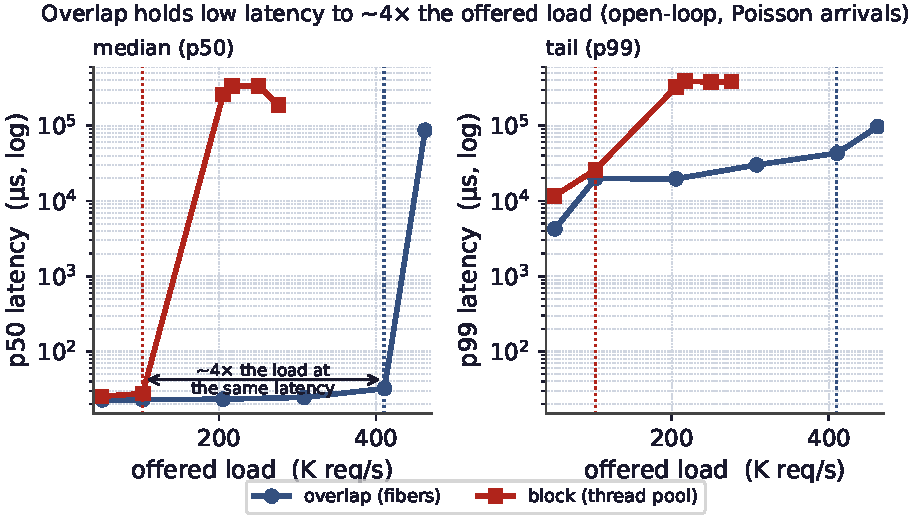
\includegraphics[width=0.86\linewidth]{figs/fig_latency.pdf}
  \caption{Latency under load (measured, open-loop Poisson arrivals, \texttt{runtime/openloop.csv}).
    Blocking on the offload drives both median (p50, left) and tail (p99, right) latency up at its
    saturation point near $103$\,K req/s, while overlapping holds low latency to roughly $4\times$
    that offered load (knee near $410$\,K req/s) before its own. Overlap is a latency win, not only a
    throughput win.}
  \label{fig:latency}
\end{figure}

\paragraph{Offload weight and the two ceilings.}
Sweeping the GPU AES offload by block size on a single event loop confirms the weight dependence: no
benefit for a light block, rising monotonically toward the GPU's bandwidth for a heavy one
(Figure~\ref{fig:weight}; full table in Appendix~\ref{app:blocksize}). The ceiling is a property of the
\emph{device}: overlap recovers the utilization that blocking wastes but cannot exceed device
throughput. A \emph{latency-bound} offload lifts that ceiling, because its device is not saturated and
many requests can be in flight at once. With our real RSA-2048 remote signer ($821$\,\textmu s
round-trip) the same Python server reaches $3.53\times$---but \emph{not} the order of magnitude a deep
queue could in principle give, because the bottleneck simply moves to the server's own overlap
capacity (the \texttt{asyncio}/GIL executor keeps only $\sim$$7$ requests truly in flight). Real
overlap is thus bounded at \emph{both} ends, by device throughput and by the concurrency the server can
express; across our servers and offloads it lands at $1.2$--$5\times$.

\paragraph{Databases.}
A process- or thread-per-connection database already overlaps offloads \emph{across} connections for
free (the OS runs the backends concurrently), so the only edit-addressable win is \emph{within} one
query that pipelines many offloads. With a launch-bound GPU op this intra-query pipelining is modest
(Figure~\ref{fig:spectrum}), set by the device once it is fed---the same edit, GPU, and per-row work,
with the win bounded by the device exactly as the model predicts.


% =====================================================================
\section{Discussion and Limitations}
\label{sec:discussion}

\paragraph{The walls are fundamental, and the win is bounded.}
The three walls of \S\ref{sec:transparent} are properties of where an application places behavior, not
gaps in our engineering: raw-syscall synchronization, thread identity in a register, and a workload
with no idle CPU each sit \emph{below} or \emph{around} the symbol layer a preloaded library can touch,
and they generalize to any storage engine with its own futexes, any managed runtime, and any CPU-bound
handler---which is precisely why the minimal-edit path exists. The same idle-CPU condition (Wall~3 and
Figure~\ref{fig:weight}) also bounds when overlap pays at all: when per-request CPU rivals the offload
there is little to reclaim, and the technique should not be applied.

\paragraph{Detector scope and complementarity.}
The conflict detector is a targeted safety net for the overlap hazard, not a general transactional
memory; shared state outside the monitored segments, or correctness beyond last-writer-wins, would
need stronger machinery. Finally, the two ends of the spectrum are a division of labor, not
competitors: transparent fiberization serves thread-per-connection servers with no source access, and
the minimal-edit recipe serves everything else---the event-driven bulk of modern serving best of all.


% =====================================================================
\section{Related Work}
\label{sec:related}

Our work sits at an under-occupied point in the design space (Figure~\ref{fig:positioning}): low
modification to \emph{existing} servers \emph{and} broad coverage across server types. Prior
approaches achieve one or the other, but not both. Transparent threading libraries require writing the
application in their style, point offload integrations target a single server, and async frameworks
assume a rewrite.

\begin{figure}[t]
  \centering
  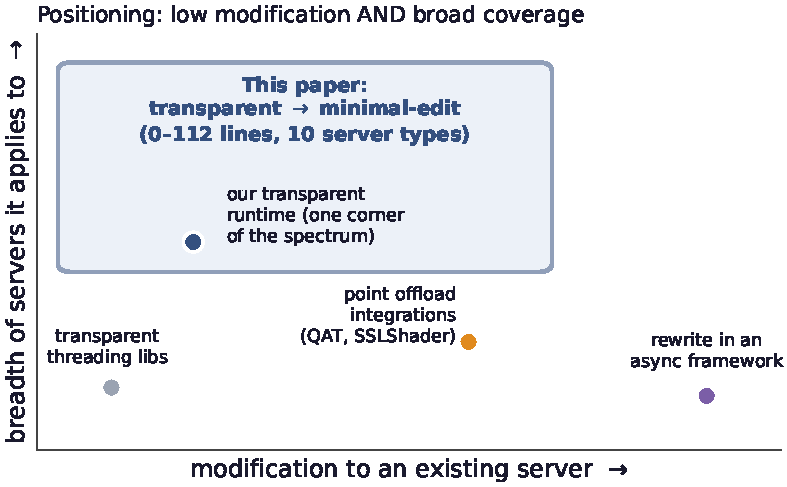
\includegraphics[width=0.86\linewidth]{figs/fig_positioning.pdf}
  \caption{Positioning. Existing approaches to overlapping work are either low-effort but narrow
    (threading libraries, of which our own transparent runtime is one) or broad but high-effort
    (point integrations, async-framework rewrites). The transparent-to-minimal-edit spectrum reaches
    the desirable region: little modification to existing servers, across many server types.}
  \label{fig:positioning}
\end{figure}

\paragraph{Threads, events, and coroutines.}
Hiding I/O latency cheaply is an old debate, between an event-driven camp that structures the server as
a state machine over an event loop at the cost of ``stack ripping'' (Flash~\cite{flash},
SEDA~\cite{seda}) and a user-level-thread camp that keeps the synchronous style and yields at blocking
points (Capriccio~\cite{capriccio}, State Threads~\cite{statethreads}, \texttt{libtask}~\cite{libtask},
core-aware Arachne~\cite{arachne}, and language-level threads such as goroutines~\cite{golang} and Java
virtual threads~\cite{loom}). Our fiber runtime is in the second lineage with a fast register-only
switch~\cite{fastwake}, but the contribution is not another threading library: it is to \emph{overlap
an accelerator offload} in servers built either way, \emph{quantify the modification cost} across real
servers, and map where the transparent form provably stops.

\paragraph{Microsecond-scale systems.}
A body of work rebuilds the OS or runtime to schedule microsecond-scale tasks efficiently: dataplane
operating systems such as IX~\cite{ix}, work-stealing for tail latency such as ZygOS~\cite{zygos}, and
core-reallocating runtimes such as Shenango~\cite{shenango}, Caladan~\cite{caladan}, and
Demikernel~\cite{demikernel}, typically over kernel-bypass I/O (DPDK~\cite{dpdk},
\texttt{io\_uring}~\cite{iouring}). They attack the same killer microsecond
problem~\cite{microsecond} but demand a new stack and rewritten applications. We instead ask how
little it costs to overlap one offload inside existing, unmodified servers; the directions are
complementary.

\paragraph{Full hardware offload.}
Another line moves the \emph{entire} datapath onto hardware: KV-Direct~\cite{kvdirect} runs a key-value
store in the NIC, ClickNP~\cite{clicknp} compiles network functions to an FPGA, iPipe~\cite{ipipe}
offloads application logic onto SmartNICs (and must itself schedule the offloaded tasks' granularity,
the dual of our problem), and GPUnet~\cite{gpunet} lets GPU code drive the network. These eliminate the
CPU's role and require rebuilding the application around the accelerator. Our target is the opposite and
far more common case: the application stays on the CPU and must hide one fine-grained step's latency
with almost no change.

\paragraph{Offload integrations and async frameworks.}
Closer to us, specific systems overlap specific offloads---TLS on GPUs (SSLShader~\cite{sslshader}),
QAT engines in nginx's async paths~\cite{qat}, and inference servers that batch GPU work
(RedisAI~\cite{redisai}, Clipper~\cite{clipper})---but each is a point integration tuned to one server
and offload. Async frameworks (libevent~\cite{libevent}, libuv~\cite{libuv}, Seastar~\cite{seastar},
\texttt{async}/\texttt{await}) and proxy offload engines (HAProxy SPOE~\cite{spoe}, Envoy
\texttt{ext\_proc}~\cite{extproc}) make overlap the default, but only if the application is written in
them from the start. We instead inject overlap into existing servers and give a \emph{predictive model}
of the win across the landscape.

\paragraph{Conflict detection.}
Page-protection dirty-tracking, software distributed shared memory~\cite{treadmarks}, and transactional
memory~\cite{htm} all detect or prevent conflicting concurrent writes. Our detector borrows the
page-protection technique but is deliberately lightweight and specialized to the one hazard overlap
introduces: a read-modify-write reordered across an offload.

\paragraph{Symbol interposition.}
The fragility of interposing versioned glibc symbols is folklore among practitioners. Our
condition-variable finding documents a concrete, reproducible instance and its fix.


% =====================================================================
\section{Conclusion}
\label{sec:conclusion}

What should the CPU do while it waits for the accelerator? It should \emph{overlap}: do other useful
work while the offload is in flight. The real question is how much an existing server must change, and
the answer is a spectrum from zero lines to about a hundred. At the zero-edit end a transparent runtime
overlaps an unmodified thread-per-connection binary, but it reaches a narrow niche, hits three
architectural walls, and cannot help the event-driven servers with the most to gain. A few lines at the
offload site, routed through a server's own concurrency mechanism, work everywhere, recovering
$1.2$--$5\times$ across ten production servers on real hardware. The win is bounded at both ends---by
the accelerator's throughput and by the server's own overlap capacity---so the order-of-magnitude wins
an unbounded model predicts do not survive real hardware, except in the purpose-built transparent
runtime ($17.3\times$). A simple model, concurrency model crossed with offload weight, predicts both
the speedup and the code cost in advance, and a transparent conflict detector keeps overlap correct
when it touches shared state. The result is a practical recipe, and a map, for hiding fine-grained
accelerator-offload latency in the servers that run online services today.


\section*{Acknowledgements}
This paper began as a draft written during the author's internship at Microsoft Research in 2017.
Nine years later, with the help of Pine Copilot and Claude Code, the author finally brought it to completion.
The work was produced using Pine Copilot's voice-directed \emph{whisper coding} workflow, in which the authors specify, discuss, and review the work by voice while a coding agent---Claude Code with Claude Opus 4.8---carries out the planning, coding, experiments, and paper writing.
We thank BSQL Networking for hosting the NVIDIA RTX PRO 6000 GPU.


% =====================================================================
\appendix
\section{AES Block-Size Sweep (detailed values)}
\label{app:blocksize}

Table~\ref{tab:blocksize} gives the full per-size measurements behind the offload-weight curve of
Figure~\ref{fig:weight}, all on a real GPU on an \emph{idle} device (no co-tenant compute), driving a
single-event-loop server (Python \texttt{asyncio} with a $32$-thread executor) at $50$ concurrent
clients. The AES block size is swept over consecutive powers of two from $4$\,KiB to $8$\,MiB. For
each we report the measured single-op GPU latency (one offload in flight), the synchronous and
asynchronous throughput, and their ratio. The speedup grows monotonically from $1.24\times$ at
$4$\,KiB (launch-bound: the offload is tens of microseconds, on the order of the server's own
per-request work, so there is little to overlap) to $5.41\times$ at $8$\,MiB (the offload is
bandwidth-bound at $\sim$$2.3$\,ms, so overlapping it across requests reclaims most of the wait), up
to the GPU's throughput ceiling.

\begin{table}[h]
  \centering
  \begin{tabular}{rrrrr}
    \toprule
    block size & GPU latency (\textmu s) & sync (req/s) & async (req/s) & speedup \\
    \midrule
    4\,KiB   & 46.4   & 3750 & 4667 & $1.24\times$ \\
    8\,KiB   & 47.0   & 3688 & 4650 & $1.26\times$ \\
    16\,KiB  & 51.4   & 3657 & 4573 & $1.25\times$ \\
    32\,KiB  & 60.3   & 3501 & 4371 & $1.25\times$ \\
    64\,KiB  & 70.2   & 3326 & 4355 & $1.31\times$ \\
    128\,KiB & 92.7   & 2970 & 4218 & $1.42\times$ \\
    256\,KiB & 126.5  & 2706 & 4128 & $1.53\times$ \\
    512\,KiB & 191.8  & 2454 & 4494 & $1.83\times$ \\
    1\,MiB   & 361.6  & 1538 & 3644 & $2.37\times$ \\
    2\,MiB   & 653.6  & 966  & 2858 & $2.96\times$ \\
    4\,MiB   & 1188.1 & 506  & 1937 & $3.83\times$ \\
    8\,MiB   & 2258.6 & 227  & 1228 & $5.41\times$ \\
    \bottomrule
  \end{tabular}
  \caption{Real-GPU AES block-size sweep on a single-event-loop server (idle GPU). Source:
    \texttt{transparent-runtime/apps/aes\_blocksize\_py\_results.csv}.}
  \label{tab:blocksize}
\end{table}


% =====================================================================
\section{Interposition Obstacles for the Transparent Runtime}
\label{app:obstacles}

Beyond the symbol-versioning hazard of \S\ref{sec:transparent} (Figure~\ref{fig:condsweep}), running
stock binaries under the \texttt{LD\_PRELOAD} fiber runtime surfaced four lesser obstacles. Each was
resolved once and is recorded here because any threading-interposing tool will meet them.

\begin{itemize}[leftmargin=1.4em,itemsep=2pt,topsep=2pt]
  \item \textbf{Alternate I/O entry points.} A server may do its socket I/O through
    \texttt{recv}/\texttt{send}/\texttt{poll} rather than \texttt{read}/\texttt{write}, so every
    blocking entry point the application can reach must be interposed to yield the fiber.
  \item \textbf{Real-thread identity.} \texttt{pthread\_self} must return the genuine OS thread
    identity, because the C library's stack-bounds logic relies on it; returning a per-fiber value
    breaks libc internals.
  \item \textbf{Carrier re-establishment after \texttt{fork}.} A daemon that forks drops the carrier
    thread in the child, which must be re-established before any fiber can run.
  \item \textbf{Priority inversion.} Pinning the carrier to a real-time priority can invert priorities
    against a lock holder running at normal priority, stalling the carrier.
\end{itemize}
